\documentclass[11pt,titlepage,oneside,openany]{book}
\usepackage{times}

\usepackage{comment}
\usepackage{graphicx}
\usepackage{latexsym}
\usepackage{amsmath}
\usepackage{amssymb}

\usepackage{ntheorem}

\usepackage{tabularx}

\usepackage{multirow}

\usepackage{algorithm}
\usepackage{algorithmic}

\usepackage{spverbatim}

\usepackage[colorlinks=false,linkcolor=black,urlcolor=black,bookmarksopen=true]{hyperref}
\usepackage{bookmark}

\newtheorem{definition}{Definition}
\newtheorem{proposition}{Proposition}

\renewcommand{\algorithmiccomment}[1]{\ensuremath{\rhd} \textit{#1}}
\def\MYCALL#1#2{{\small\textsc{#1}}(\textup{#2})}
\def\MYSET#1{\scshape{#1}}
\def\MYAND{\textbf{ and }}
\def\MYOR{\textbf{ or }}
\def\MYNOT{\textbf{ not }}
\def\MYTHROW{\textbf{ throw }}
\def\MYBREAK{\textbf{break }}
\def\MYEXCEPT#1{\scshape{#1}}
\def\MYTO{\textbf{ to }}
\def\MYNIL{\textsc{Nil}}
\def\MYUNKNOWN{ unknown }

\def\INT{{\mathcal I}}
\def\ONT{{\mathcal O}}
\def\SEM{{\mathcal S}}
\def\ALI{{\mathcal A}}
\def\USE{{\mathcal U}}
\def\CON{{\mathcal C}}
\def\DIA{\Delta}

\def\MUP{{\mathcal M}}
\def\MIP{{\mathcal M}}

\newcommand{\cc}[2]{\mathit{#1}\hspace{-1pt} \# \hspace{-1pt} \mathit{#2}}
\newcommand{\cx}[1]{\mathit{#1}}

\def\MER#1#2#3#4{#1 \cup_{#3}^{#2} #4}
\def\MUPALL#1#2#3#4#5{\textit{MUPS}_{#1}\left(#2, #3, #4, #5\right)}
\def\MIPALL#1#2{\textit{MIPS}_{#1}\left(#2\right)}

\begin{document}

\begin{titlepage}
	\vspace*{2cm}
  \begin{center}
   {\Large Wikidata: A Free Collaborative Knowledge Graph\\}
   \vspace{2cm} 
   {Knowledge Graphs Seminar\\}
   \vspace{2cm}
   {presented by\\
    Nahor Gebretensae\\
   }
   \vspace{1cm} 
   {submitted to the\\
    Data and Web Science Group\\
    Prof.\ Dr.\ Heiko Paulheim\\
    University of Mannheim\\} \vspace{2cm}
   {June 2019}
  \end{center}
\end{titlepage}

\pagenumbering{roman}

\tableofcontents

\listoffigures

\listoftables

\newpage

\pagenumbering{arabic}

\chapter{Introduction}
\label{chap:intro}

\section{Motivation}
Wikipedia was originally conceived in 2001 as a text-based resource. But the amount of structured data such as numbers, dates, coordinates, and many types of relationships, from family trees to species taxonomy, has steadily increased in Wikipedia. According to the Wikimedia Foundation’ vision of giving everyone access to knowledge, Wikipedia must contain data that can be searched, analyzed, and reused. But most of the data in Wikipedia cannot be accessed through query services or by downloading data dumps. The obvious divide between vision and reality lies in the fact that Wikipedia’s data is contained in over 30 million Wikipedia articles in about 300 languages. In addition, the information in the various language versions of Wikipedia articles may differ. Wikidata, a sister project of Wikipedia, was launched in October 2012 to clean up this structured data and store it in a central location. Wikidata is a kind of multilingual Wikipedia for data \cite{AFCK01}.
\\
\\
Wikidata is characterized by the following features:
\begin{itemize}
	\item \textbf{Open editing:} The extension and processing of the stored information is possible without creating an account via a forms-based interface \cite{AFCK01}.
	\item \textbf{Community control:} The community of contributors controls the schema of the data and the actual data. Only editors can create elements in Wikidata and link them to Wikipedia articles \cite{AFCK01}.
	\item \textbf{Plurality:} Because many facts are controversial or uncertain, Wikidata allows conflicting data to coexist and offers the possibility to administer plurality \cite{AFCK01}.
	\item \textbf{Secondary data:} Wikidata collects facts from primary sources and publishes them with references to these sources \cite{AFCK01}.
	\item \textbf{Multilingual data:} Wikidata is multilingual by design as most data such as numbers, dates, and coordinates have a universal meaning and are not tied to any language \cite{AFCK01}.
	\item \textbf{Easy access:} Wikidata's goal is also to allow the use of data outside Wikipedia in external applications. The data is exported via web services in various formats, including RDF \cite{AFCK01}.
	\item \textbf{Continuous evolution:} Wikidata is not a fully developed system that is presented to the world but is implemented step by step \cite{AFCK01}.
\end{itemize}

\section{Outline}
To give an overview of Wikidata, the content of this paper is mainly based on five works discussing different Wikidata topics. In \textit{Wikidata: A Free Collaborative Knowledgebase} \cite{AFCK01}, Vrandečić et al. describe the architecture, name possible use cases, and show development perspectives of Wikidata. Ehrlinger et al.'s \textit{Towards a Definition of Knowledge Graphs} \cite{TDKG01} defines the term knowledge graph, taking into account its history and diversity in interpretation and use. Malyshev et al.'s \textit{Getting the Most Out of Wikidata: Semantic Technology Usage in Wikipedia's Knowledge Graph} \cite{Malyshev2018GettingTM} analyzes the underlying infrastructure that enables the use of SPARQL endpoints and access to RDF dumps. Tanon et al.'s \textit{From Freebase to Wikidata: The Great Migration} \cite{Tanon2016FromFT} analyzes transfer efforts and data mapping challenges. Ringler et al.'s \textit{One Knowledge Graph to Rule Them All?} \cite{Ringler2017OneKG} evaluates the strengths and weaknesses of various knowledge graphs, including Wikidata, when it comes to applications in different domains.
\\
\\
\textit{Chapter~\ref{chap:kg}, \nameref{chap:kg}}, defines the term knowledge graph. \textit{Chapter~\ref{chap:wikidata}, \nameref{chap:wikidata}}, based on scientific papers, describes the architecture of Wikidata, and the following \textit{Chapter~\ref{chap:semwebtech}, \nameref{chap:semwebtech}}, analyzes the underlying infrastructure that enables the use of SPARQL endpoints and access to RDF dumps. \textit{Chapter~\ref{chap:migration}, \nameref{chap:migration}}, analyzes the transfer efforts of data from Freebase to Wikidata. \textit{Chapter~\ref{chap:applications}, \nameref{chap:applications}}, discusses the commonalities and particularities of the different knowledge graphs and assesses the strengths and weaknesses of Wikidata when it comes to applications in different domains. The paper concludes in \textit{Chapter~\ref{chap:prospects}, \nameref{chap:prospects}}, with discussions on future research waiting for Wikidata.

\chapter{Definition of Knowledge Graphs}
\label{chap:kg}
The term knowledge graph has often been used in close association with Semantic Web Technologies, Linked Data, Large-Scale Data Analytics, and Cloud Computing. A variety of interpretations of the term knowledge graph hindered the development of a common definition. But a clear definition is necessary for a common understanding of the benefits, drawbacks, and possible applications of a knowledge graph. \cite{TDKG01}
This chapter is mainly based on the work of Ehrlinger et al., \textit{Towards a Definition of Knowledge Graphs}, \cite{TDKG01} and defines the term knowledge graph taking into account its history and diversity in interpretations and use.
\\
\\

\section{First Occurrences of the Term Knowledge Graph} 
The term knowledge graph was first used in the 1980s by researchers from the University of Groningen and the University of Twente to describe their knowledge-based system that integrates knowledge from various sources to represent the natural language \cite{a4591467cd12418da0e44ac054c07cf8}. These knowledge graphs had a limited number of relationships and focused heavily on qualitative modeling. The above-mentioned understanding of the term Knowledge Graph, however, contradicts the idea of the Knowledge Graph that has been discussed since the introduction of the Google Knowledge Graph \cite{TDKG01}.
\\
\\

\section{Google Knowledge Graph} 
In 2012, Google introduced the Knowledge Graph as an extension of Google's search capabilities. Instead of assigning strings, the knowledge graph facilitates the search for ``things'' or real-world objects \cite{TDKG06}. This frequently quoted blog entry by Google \cite{TDKG06} describes only an extension of the own search engine but does not define the term knowledge graph. Following the publication of the blog entry, the term Knowledge Graph has been used for a number of applications, including DBpedia, YAGO, Freebase, Wikidata, and OpenCyc \cite{LDQ01}. However, all these applications differ in their characteristics, architecture, purpose, and technology used. The lowest common denominator of these applications is the use of Liked Data \cite{TDKG01}.
\\
\\ 

\section{Terminological Analysis and Definition}
\textbf{Ambiguity.} The terms knowledge graph and knowledge base are often used interchangeably. Knowledge Vault and Google Knowledge Graph have been called knowledge bases by their creators \cite{Dong2014KnowledgeVA}. The term \textit{knowledge graph} is used as a synonym for \textit{knowledge base}, which is often used as a synonym for \textit{ontology}. For example, YAGO, an ontology with its name, is also referred to as a knowledge base \cite{Ringler2017OneKG} or knowledge graph \cite{TDKG02}. Because of these ambiguities, it is necessary to explicitly state the differences between the terms. In order to be able to distinguish the terms from each other, they must first be clearly defined \cite{TDKG01}.
\\
\\
\textbf{Knowledge-based systems.} The publication by Akerkar et al., \textit{Knowledge-Based Systems} \cite{TDKG03}, states that knowledge-based systems use artificial intelligence to solve problems. Knowledge-based systems consist of a knowledge base and an inference engine. A knowledge base is a dataset of formal semantics that contains different types of knowledge, such as rules, facts, axioms, definitions, statements, and primitives \cite{TDKG03}. Inference engines or reasoning engines can derive conclusions from known facts \cite{Feilmayr2016AnAO}.  
\\
\\
\textbf{Ontology.} Since ontologies enable semantic modeling of knowledge, they are used as a knowledge base in artificial intelligence applications in the context of knowledge-based systems. Ontologies can then be used to derive conclusions from known facts \cite{TDKG05}. According to Shvaiko and Euzenat \cite{Shvaiko2013OntologyMS}, an ontology does not differ from a knowledge base.
\\
\\
\textbf{Knowledge Graph.} Since size is an important feature of knowledge graphs, knowledge graphs could be described as large ontologies. However, knowledge graphs can also be differentiated by advanced ontologies functions. For example, in contrast to ontologies, knowledge graphs have an integrated reasoner that can be used to derive new knowledge. This leads to the conclusion that a knowledge graph is a knowledge-based system, which in turn consists of a knowledge base and a reasoning machine. But Knowledge Graphs allow in addition the collection, extraction, and integration of information from external sources. This adds a concept of an integration system to a Knowledge-Based System. As Figure \ref{fig:knowledge-graph-architecture} shows, a knowledge graph captures and integrates information in an ontology and uses a reasoner to derive new knowledge. Most open-source applications implement the integration aspect of knowledge graphs using linked data \cite{TDKG01}.
\\
\\ 

\begin{figure}
	\begin{center}
	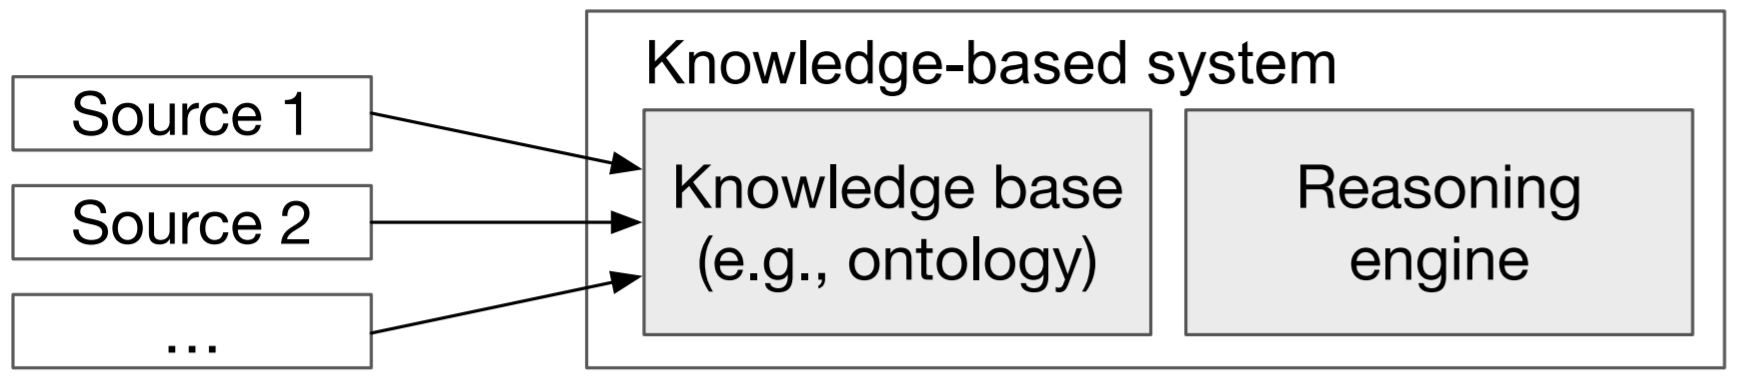
\includegraphics[width=13cm]{./figures/knowledge-graph-architecture.png}
	\caption[Architecture of a knowledge graph]{Architecture of a knowledge graph \cite{TDKG01}}
	\label{fig:knowledge-graph-architecture}
	\end{center}
\end{figure}

\chapter{Data Model}
\label{chap:wikidata}
This chapter is mainly based on the work \textit{Wikidata: A Free Collaborative Knowledgebase} \cite{AFCK01} by Vrandečić et al. and defines the data model used by Wikidata.
\\
\\
Like Wikipedia, Wikidata is organized in pages. Every subject in Wikidata, which contains structured data, is called an \textit{entity}, and every \textit{entity} has a page. The data model distinguishes between two types of entities: \textit{items} and \textit{properties} \cite{Erxleben2014IntroducingWT}.
\\
\\

\section{Wikidata Item}
For Wikidata to be truly multilingual, every object in every language must be one and the same. Wikipedia uses language links to link articles in any language, resulting in a quadratic number of links. However, it would be much better to manage language links in a single location. Therefore, for each Wikipedia article, a page was created in Wikidata containing links to related Wikipedia articles in all languages. Initially, these pages are known as \textit{items}. The Wikidata community has created bots to move language links from Wikipedia to Wikidata. However, you can still add custom links to Wikipedia articles \cite{AFCK01}.
\\
\\
Each item represents a coherent concept like a person, a device or a chemical substance \cite{Heindorf2016VandalismDI} and is identified by an opaque identifier, which gets automatically created and cannot be changed later on. The item identifier starts with "Q" followed by a number \cite{Erxleben2014IntroducingWT}. The content of an item consists of head and body parts. The head consists of the \textit{label}, a short \textit{description} and a list of \textit{aliases} \cite{Heindorf2016VandalismDI}, which are collectively known as \textit{terms}. Terms are mainly used to find and to display items \cite{Erxleben2014IntroducingWT}. Moreover, they can be present in up to 291 supported languages. The body consists of a list of \textit{statements} and a list of \textit{site links} \cite{Heindorf2016VandalismDI}. Site links are links to pages about the entity in other Wikimedia projects (e.g. Wikipedia) \cite{Erxleben2014IntroducingWT}.
\\
\\
\textbf{Wikidata statement. } Statements encode all of the structural knowledge of Wikipedia and are composed of subject-predicate-object triples, where, an \textit{item} corresponds to the subject, a \textit{property} to the predicate and \textit{value} to the object \cite{Heindorf2016VandalismDI}. Main property-value-pairs are also called \textit{claim}. A claim consists of one main property-value pair and has one or more references \cite{Tanon2016FromFT}.
\\
\\
\textbf{External identifiers. } Wikidata allows the integration of external identifiers from other databases and authority controls, such as: the International Standard Name Identifier (ISNI), CALIS (China Academic Library and Information System), IATA (International Air Transport Association), HURDAT (North Atlantic Basin's Hurricane Database), and MusicBrainz. These external identifiers can then be used to obtain data from other sources \cite{AFCK01}.
\\
\\
\textbf{Data access. } The data is provided in different ways. For example, per-item exports are available in JSON, XML, RDF, and other formats. Full data dumps are only generated at fixed intervals. This follows the Linked Data standards for publishing data, making Wikidata a part of the Semantic Web \cite{AFCK01}.
\\
\\

\section{Wikidata Property}
The properties are objects and have their own Wikidata pages with names, aliases, and descriptions \cite{AFCK01} and use opaque identifier starting with "P" followed by a number \cite{Erxleben2014IntroducingWT}. In addition, the data type of the property value is specified on the property pages \cite{AFCK01}. As can be seen in Table \ref{tab:wikidata-datatypes}, there are six different data types \cite{Erxleben2014IntroducingWT}. As in Figure \ref{fig:complex-statement-wikidata}, the \textit{item} "Rome" may have the \textit{property} "Population" with the \textit{value} "2,761,477" \cite{AFCK01}. 
\\
\\
\textbf{Wikidata Qualifier. } Property-value pairs are not sufficient in most cases. It is difficult to present the following information with property-value pairs: According to an estimate, the population of Rome is 2,761,477 people as of 2010. This problem can be solved by adding the property "as of" with the value "2010" and the property "method" with the value "estimation". These two properties do not refer to the element of Rome as the property "population" but to the statement that Rome has a population of 2,761,477. As can be seen in Figure \ref{fig:complex-statement-wikidata}, this creates a model in which a property pair may have multiple subordinate property-value pairs. These child property-value pairs are called \textit{qualifiers}. Qualifiers can be used to represent contextual information or ternary relationships. In addition, Wikidata allows a value or property to be unknown \cite{AFCK01}.
\\
\\
\textbf{Wikidata reference. } In Wikidata, each statement can contain a list of references to sources. The inclusion of references is in line with Wikipedia's vision of being a secondary source that does not publish its own research but collects information. References are basically a list of property-value pairs. The details of the reference modeling are set by the community. Different sources represent different ``views'', but Wikipedia's goal is to represent all ``views'', rather than choosing a true ``view''. In order to do justice to this plurality, Wikidata allows certain ``views'' to be marked as preferred. The task of classification is subject to the Community \cite{AFCK01}.
\\
\\
\begin{table}[h]
\begin{center}
\begin{footnotesize}
\begin{tabular*}{\textwidth}{|l|l|}
\hline
Datatype & Member fields and field types\\ \hline
Item & item id (IRI) \\
String & string \\
URL & URL (IRI) \\
Commons Media & article title (string) \\
Time & precision (byte), before tolerance (int), after tolerance (int), timezone off- \\
& set (int), point in time (dateTime), preferred calendar (IRI) \\ 
Global coordinates & latitude (decimal), longitude (decimal), globe (IRI), precision (decimal) \\
Quatity & value (decimal), lower bound (decimal), upper bound (decimal) \\ \hline
\end{tabular*}
\end{footnotesize}
\caption[Wikidata datatypes]{Wikidata datatypes and their member fields and field types \cite{Erxleben2014IntroducingWT}}
\label{tab:wikidata-datatypes}
\end{center}
\end{table}
\begin{figure}
	\begin{center}
	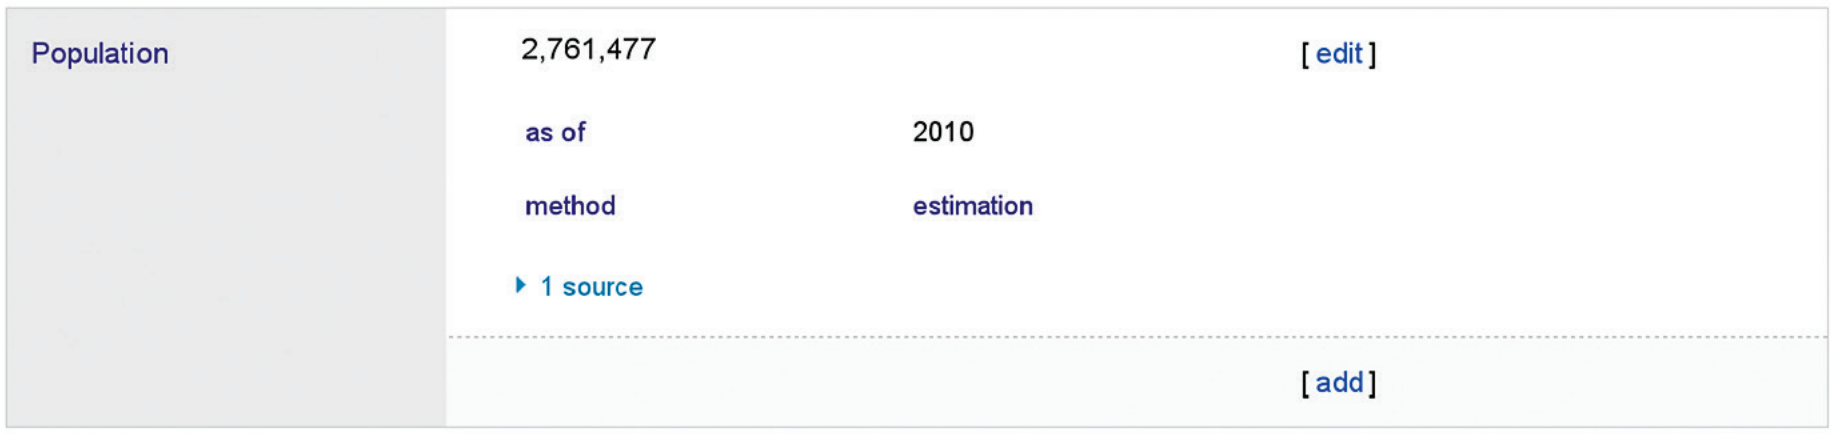
\includegraphics[width=13cm]{./figures/complex-statement-wikidata.png}
	\caption[Complex statement]{Complex statement in Wikidata \cite{AFCK01}}
	\label{fig:complex-statement-wikidata}
	\end{center}
\end{figure}

\chapter{Usage of Semantic Web Technologies}
\label{chap:semwebtech}
Wikidata is a core project for the data management strategy of the Wikimedia Foundation. The content of Wikidata consists of strings stored as character blobs in a MySQL database. The initial infrastructure with the underlying MediaWiki software is not suitable for advanced data analysis or query mechanisms. The lack of query mechanisms was, for example, a problem for editors who are trying to detect errors. Many possible solutions, including an own custom build software, were considered. To provide a powerful data sharing and retrieval service, the Wikimedia Foundation decided to build the core functionality on semantic technologies, especially RDF and SPARQL. The main reason for this decision was the accessibility of well-supported open-source tools \cite{Malyshev2018GettingTM}. This chapter is mainly based on the work \textit{Getting the Most Out of Wikidata: Semantic Technology Usage in Wikipedia's Knowledge Graph} by Malyshev et al. \cite{Malyshev2018GettingTM} and analyzes the underlying infrastructure that enables the use of SPARQL endpoints and access to RDF dumps.
\\
\\

\section{Encoding Wikidata statements in RDF}
The graph-like knowledge representation of Wikidata is very close to RDF: Properties are connecting items and data values. The difference between Wikidata and RDF is that components of the Knowledge Graph contain more information than plain RDF would allow carrying \cite{Malyshev2018GettingTM}. As explained in \textit{Chapter~\ref{chap:wikidata}, \nameref{chap:wikidata}}, Wikidata statements are not just triples but have additional qualifiers and references \cite{Erxleben2014IntroducingWT}.
\\
\\
There are two cases where a Wikidata statement can contain more information than plain RDF would allow carrying \cite{Malyshev2018GettingTM}. As can be seen from Figure \ref{fig:wikidata-statement}, Wikidata states that the item \textit{Germany} for property \textit{speed limit} has a value of \textit{100 km/h}. This Wikidata statement contains much additional information that cannot be represented in plain RDF \cite{Malyshev2018GettingTM}:
\begin{itemize}
	\item Wikidata data values often do not correspond to literals. The data value \textit{100 km/h}, for example, consists of a numerical value and a unit of measure \cite{Malyshev2018GettingTM}. 
	\item The additional qualifier \textit{valid in place} (\texttt{P3005}) illustrates the context in which the statement is valid. Such kind of nested annotation is not possible in plain RDF \cite{Malyshev2018GettingTM}. 
\end{itemize}
Therefore, complex values and annotated statements need to be represented in auxiliary nodes, which are the subject of further RDF triples, as shown in Figure \ref{fig:rdf-graph-wikidata-statement} \cite{Malyshev2018GettingTM}: Items relate to statements and statements relate to values, qualifier values and references \cite{Erxleben2014IntroducingWT}.
\\
\\
\textbf{Statement node. }As can be seen in Figure \ref{fig:rdf-graph-wikidata-statement}, the Wikidata statement in Figure \ref{fig:wikidata-statement} becomes a statement node and the data value for the property \textit{speed limit} becomes a value node. From the statement node, one can access the value node by following \texttt{psv:P3086}, the reference node by following \texttt{prov:wasDerivedFrom} or the qualifier node by following \texttt{pq:P3005} \cite{Malyshev2018GettingTM}.
\\
\\
\textbf{Value node. } The data value \textit{100 km/h} consists of a numerical value and a unit of measure. From the value node, one can access the numerical value following \texttt{quantityAmount} or the unit of measure following \texttt{quantityUnit}. It is not possible to store the unit of measure and the numerical value in one item \cite{Malyshev2018GettingTM}.
\\
\\
\textbf{Statement rank. } Ranks are built-in statement annotations, which simplify basic filtering. Statements can contain one of the following ranks: \textit{normal} (default), \textit{preferred} or \textit{deprecated}. Statement ranks are useful when there are multiple statements for one property. The city of Rome, for example, has multiple population numbers at different times. But the most recent population number has the statement rank preferred. This makes it possible to determine the current population with a simple SPARQL query \cite{Malyshev2018GettingTM}.
\\
\\

\begin{figure}
	\begin{center}
	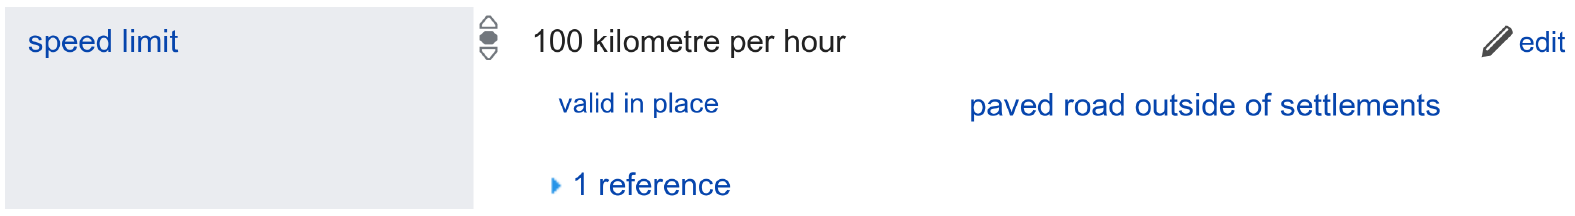
\includegraphics[width=13cm]{./figures/wikidata-statement.png}
	\caption[Wikidata statement]{Wikidata statement \cite{Malyshev2018GettingTM}}
	\label{fig:wikidata-statement}
	\end{center}
\end{figure}
\begin{figure}
	\begin{center}
	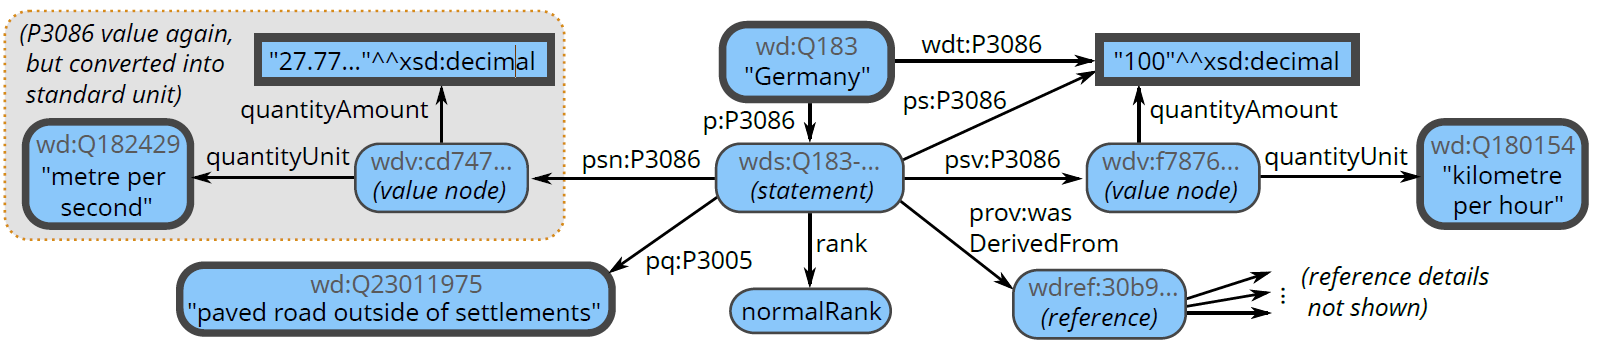
\includegraphics[width=13cm]{./figures/rdf-graph-wikidata-statement.png}
	\caption[RDF graph for Wikidata statement]{RDF graph for the statement from Figure \ref{fig:wikidata-statement}, with added annotations and highlights for readability \cite{Malyshev2018GettingTM}}
	\label{fig:rdf-graph-wikidata-statement}
	\end{center}
\end{figure}

\section{Wikidata RDF Exports and Query Service} 
The Wikimedia Foundation creates weekly RDF dumps. There are complete dumps of all triples and smaller dumps with simplified triples. The dumps are generated by Wikibase, the software used to run Wikidata, and the RDF is generated by the PHP library Purtle \cite{Malyshev2018GettingTM}.
\\
\\
The SPARQL query service was introduced in 2015 and built on top of the BlazeGraph RDF store and graph database. The user interface has a forms-based query editor and a SPARQL input. The user interface allows the user to autocomplete Wikidata entries \cite{Malyshev2018GettingTM}. 
\\
\\

\section{Is Wikidata a knowledge base?}
According to Vrandečić et al.`s \cite{AFCK01}, Wikidata is a knowledge base. But according to Ehrlinger et al.`s \cite{TDKG01}, Wikidata is not just a knowledge base. Since Wikidata captures and integrates information from external sources, using external identifiers, in a knowledge base and uses a reasoner, the SPARQL Query Service,  to derive new knowledge \cite{Malyshev2018GettingTM}, Wikidata is a knowledge graph \cite{TDKG01}.

\chapter{From Freebase to Wikidata}
\label{chap:migration}
Freebase is an open and collaborative knowledge base which was launched in 2007 by Metaweb and acquired in 2010 by Google. In 2014, Google decided to shut down Freebase and offered to transfer the content of Freebase to Wikidata \cite{Tanon2016FromFT}. 
\\
\\
Data migration is challenging since both knowledge bases do not have a similar design and require a mapping between their structures. Moreover, cultural differences between the participating communities must be taken into account. Freebase and Wikidata communities have different backgrounds, goals, understandings of their tasks, and requirements regarding their data \cite{Tanon2016FromFT}. 
\\
\\
This chapter is mainly based on the work \textit{From Freebase to Wikidata: The Great Migration} by Tanon et al. \cite{Tanon2016FromFT} and analyzes transfer efforts and data mapping challenges.
\\
\\

\section{Differences Between Freebase and Wikidata}
Freebase is based on the concepts of \textit{objects}, \textit{facts}, \textit{types}, and \textit{properties}. Each object has an identifier which is called \textit{mid} and one or more \texttt{types}. The properties of these types provide the facts \cite{Tanon2016FromFT}. 
\\
\\
As can be seen from Figure \ref{fig:exemplary-compound-value-type-freebase}, \textit{Barack Obama}, for example, is an object that has the mid \textit{/m/02mjmr} and the type \textit{/government/us-president}. This type allows the entity to have a fact with the property \textit{/government/us-president/presidency-number} and \textit{44} as the value \cite{Tanon2016FromFT}.
\\
\\
As shown in Figure \ref{fig:exemplary-compound-value-type-freebase}, Freebase uses Compound Value Types to represent n-ary relationships. CVT values are objects and can have types. Most non-CVT objects are topics \cite{Tanon2016FromFT}.
\\
\\
Wikidata, on the other hand, is built on the notion of \textit{item} and \textit{statement}. An item represents an entity and has an identifier, labels, a description, aliases in multiple languages, additional statements, and links to pages about the entity in other Wikimedia projects (e.g. Wikipedia). Wikidata does not represent true facts but displays claims from different sources which may contradict each other \cite{Tanon2016FromFT}.
\\
\\

\begin{figure}
	\begin{center}
	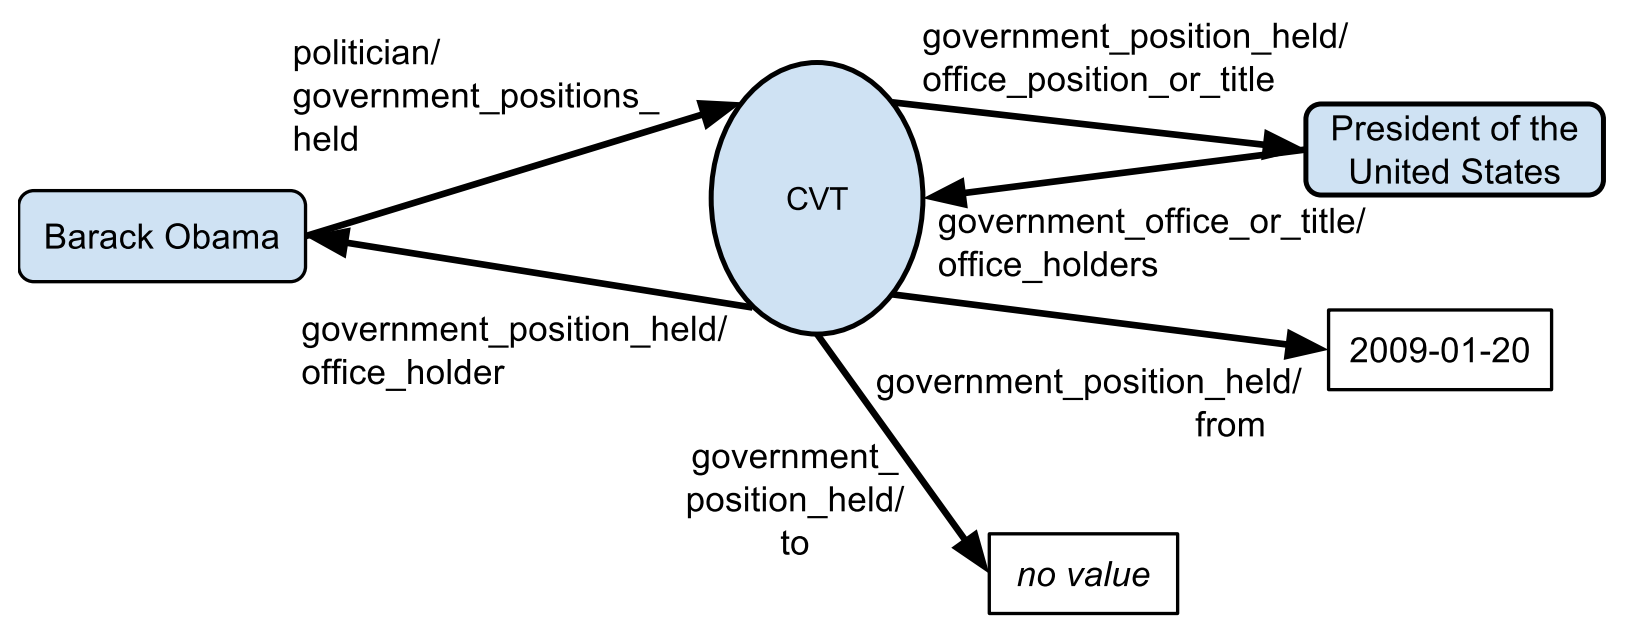
\includegraphics[width=13cm]{./figures/exemplary-compound-value-type-freebase.png}
	\caption[Exemplary Compound Value Type (CVT) in Freebase]{Exemplary Compound Value Type (CVT) in Freebase \cite{Tanon2016FromFT}}
	\label{fig:exemplary-compound-value-type-freebase}
	\end{center}
\end{figure}

\section{Challenges of Migration}
The migration of Freebase to Wikidata entails a number of technical and non-technical challenges, which are discussed below \cite{Tanon2016FromFT}.
\\
\\
\textbf{Licensing. } Freebase is released under the Creative Commons Attribution (CC BY 2.5) license, which allows adding content to the knowledge graph for which Google does not own the copyright. Since Wikidata is published under the Creative Commons 0 (CC0 1.0) license, which effectively places the data into the public domain, some content of the Freebase Knowledge Graph must be filtered \cite{Tanon2016FromFT}.
\\
\\
\textbf{References. } Unlike Wikidata, Freebase usually has no references saved. To provide Wikidata with references for the facts in Freebase, data from the Google Knowledge Graph has been reused. Google Knowledge Graph extracts facts from the Web. The extracted facts are usually correct and accurate. However, the pages from which the facts are extracted do not conform to Wikidata requirements for reliable references. Therefore, it was necessary to filter the references using a domain blacklist \cite{Tanon2016FromFT}.
\\
\\
\textbf{Data quality. } The overall quality of the data in Freebase was not sufficient for a direct import. The city Boston, for example, had the type \textit{/people/person}. For this reason, a crowd-sourced human curation was required. The \textit{Primary Source Tool} was used for this task. The tool displays the curation's Freebase statements that can be added to the currently displayed Wikidata item \cite{Tanon2016FromFT}. 
\\
\\
\textbf{Long-term maintenance. } The Wikidata community is responsible for collecting and maintaining the data to protect it from vandalism. But an increased amount of data also increases the maintenance. Therefore, an increase of the amount of data must be accompanied by an increase in the number of editors or the use of tools that allow editors to work more effectively. The \textit{Primary Source Tool} has helped to make existing editors more effective and lowered the barriers for Community members to become editors \cite{Tanon2016FromFT}.
\\
\\
\textbf{Data Topic Mappings. } If a Wikidata item and Freebase topic contain links to the same Wikipedia page, they are assumed to describe the same topic. This type of mapping is considered very accurate. A second mapping approach was developed by Samsung. It is based on the same idea and assigns a Freebase topic to a Wikidata item even if there is only one shared link to a Wikipedia page \cite{Tanon2016FromFT}. 
\\
\\
External identifiers from third-party databases shared by Freebase and Wikidata can be used for reconciliation \cite{Tanon2016FromFT}. 
\\
\\
With the above approaches, most topics were able to be automatically mapped. The mapped topics have an average of 13.9 facts, while the unmapped topics had an average of 5.7 facts. This indicates that the most important topics have been mapped since important topics usually contain more facts \cite{Tanon2016FromFT}.
\\
\\
\textbf{Data Property Mapping. } With the help of the Community, 360 properties were manually mapped between Wikidata and Freebase. However, mapping CVT is more complicated. In order to map CVT, it must first be evaluated which of the CVT properties should be used as the main value. The other properties are mapped to qualifiers \cite{Tanon2016FromFT}. 
\\
\\
As can be seen from Figure \ref{fig:wikidata-statement-freebase-compound-value-type}, the Wikidata \textit{position held} property maps the Freebase properties \textit{/politician/government-positions-held} and \textit{/government-position-held/office-position-or-title}. The Wikidata property \textit{start time} maps the Freebase property \textit{/government-position-held/from} \cite{Tanon2016FromFT}.
\\
\\

\begin{figure}
	\begin{center}
	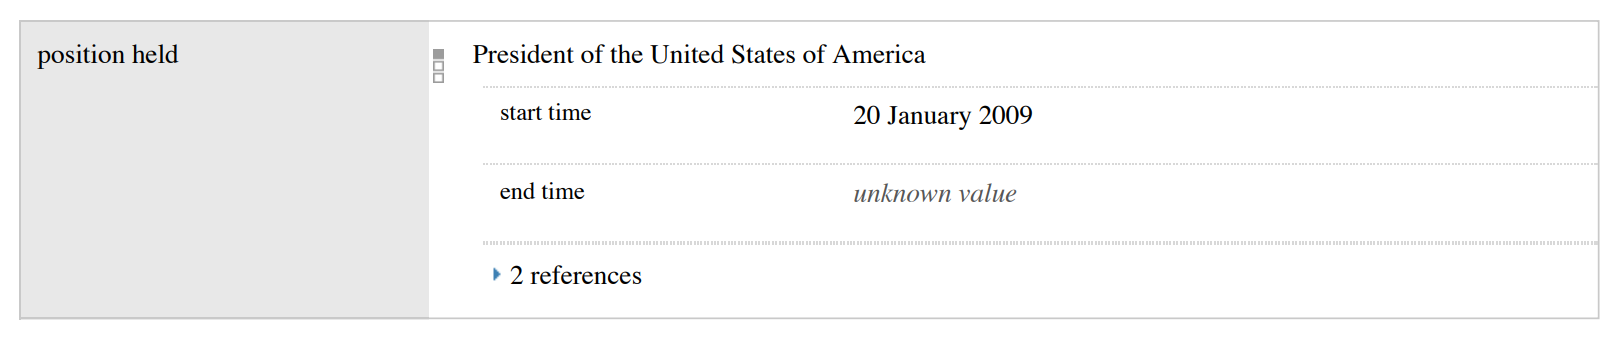
\includegraphics[width=13cm]{./figures/wikidata-statement-freebase-compound-value-type.png}
	\caption[Wikidata statement for a Freebase Compound Value Type (CVT)]{Wikidata statement for a Freebase Compound Value Type (CVT) \cite{Tanon2016FromFT}. See Figure \ref{fig:exemplary-compound-value-type-freebase} for comparison.}
	\label{fig:wikidata-statement-freebase-compound-value-type}
	\end{center}
\end{figure}

\chapter{Wikidata Applications}
\label{chap:applications}
Knowledge Graphs are almost not interchangeable. Each of them has its strengths and weaknesses when it comes to applications in different domains. Choosing a knowledge graph for a task is therefore not an easy task \cite{Ringler2017OneKG}. According to Ringler et al.'s \textit{One Knowledge Graph to Rule Them All?} \cite{Ringler2017OneKG}, there are no guidelines or best practices on choosing the right knowledge graph. This chapter quantifies differences and identifies the parts overlapping with other public knowledge graphs \cite{Ringler2017OneKG}.
\\
\\

\section{Public Knowledge Graphs on the Web}
There are various public knowledge graphs, including DBpedia, YAGO, Wikidata, OpenCyc, and NELL \cite{Ringler2017OneKG}. The knowledge graphs DBpedia and YAGO were created by extracting information from Wikipedia \cite{Lehmann2015DBpediaA}\cite{Suchanek2007YagoAC}. Wikidata, on the other hand, is a manually curated knowledge graph \cite{AFCK01}. Wikidata does also imports other datasets as well as the discontinued knowledge graph Freebase. OpenCyc is curated by experts, and NELL uses knowledge from the Web \cite{Ringler2017OneKG}.
\\
\\
\textbf{Number of instances. } An instance is the manifestation of a class \cite{instancedef}. DBpedia and YAGO have the same number of instances because an instance is always created for a Wikipedia page. Since \textit{Wikidata} is edited by a community and other datasets are imported, it contains three times as many instances \cite{Ringler2017OneKG}. 
\\
\\
\textbf{Number of axioms. } An axiom is a statement that is undoubtedly considered true \cite{axiomdef}. The fact that YAGO, despite the small number of instances, has a high number of axioms, as in Wikidata, indicates a high degree of detail. OpenCyc and NELL are much smaller than the other knowledge graphs, and the small number of axioms indicates a low density \cite{Ringler2017OneKG}. 
\\
\\
\textbf{Number of classes. } The number of classes also varies greatly between the knowledge graphs. For example, YAGO automatically generates fine-grained classes based on Wikipedia categories. Therefore, YAGO has a comparatively high number of classes. Other knowledge graphs like DBpedia or NELL have manually curated ontologies and therefore much fewer classes \cite{Ringler2017OneKG}. 
\\
\\

\begin{table}[h]
\begin{center}
\begin{footnotesize}
\begin{tabular*}{\textwidth}{|l|l|l|l|l|l|}
\hline
KG & DBpedia & YAGO & Wikidata & OpenCyc & NELL \\ \hline
Version & 2016-04 & YAGO3 & 2016-08-01 & 2016-09-05 & 08m.995 \\ \hline
\# of instances & 5,109,800 & 5,130,031 & 17,581,152 & 118,125 & 1,974,297 \\
\# of axioms & 397,831,457 & 1,435,808,056 & 1,633,309,138 & 2,413,894 & 3,402,971 \\
Avg. indegree & 13.52 & 17.44 & 9.83 & 10.03 & 5.33 \\
Avg. outdegree & 47.55 & 101.86 & 41.25 & 9.23 & 1.25 \\ 
\# of classes & 754 & 756,331 & 30,765 & 116,822 & 290 \\
\# of relations & 3,555 & 93,659 & 11,053 & 165 & 1,334 \\ \hline
\end{tabular*}
\end{footnotesize}
\caption[Properties of knowledge graphs]{Global properties of public knowledge graphs \cite{Ringler2017OneKG}}
\label{tab:propertiesKG}
\end{center}
\end{table}

\section{Experimental Evaluation: Category-Specific Analysis}
Riedlinger et al. \cite{Ringler2017OneKG} tried to quantify the differences between the knowledge graphs. As can be seen from Figure \ref{fig:category-specific-analysis}, 25 classes were chosen to compare the knowledge graphs DBpedia (D), YAGO (Y), Wikidata (W), OpenCyc (O), and NELL (N). In comparison, the number of instances, the number of indegrees, and the number of outdegrees were important metrics \cite{Ringler2017OneKG}. 
\\
\\
Outdegree is the number of edges directed out of a vertex in a directed graph. Indegree is the number of edges that are directed to a vertex in a directed graph \cite{Ringler2017OneKG}.
\\
\\
\textbf{Number of instances.} The number of instances indicates that Wikidata contains significantly more people, music albums, and books than other knowledge graphs. Although Wikidata has many instances of music albums, classes such as songs are not well represented. Although DBpedia and YAGO are derived from Wikipedia, the number of events in YAGO is higher. On the other hand, DBpedia has more information on settlements \cite{Ringler2017OneKG}.
\\
\\
\textbf{Average indegree and outdegree.} Furthermore, Wikidata has a higher level of detail for chemical substances and countries, which can be recognized by the number of indegrees and outdegrees. \cite{Ringler2017OneKG}.
\\
\\

\begin{figure}
	\begin{center}
	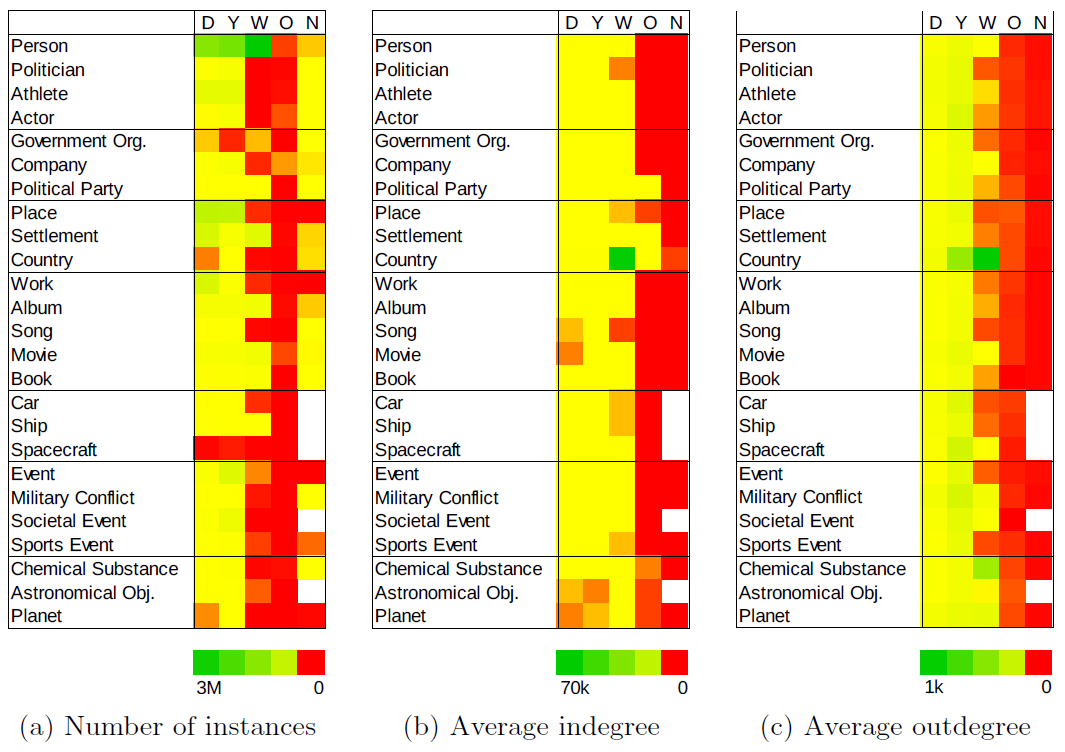
\includegraphics[width=13cm]{./figures/category-specific-analysis.png}
	\caption[Category-specific analysis]{Category-specific analysis \cite{Ringler2017OneKG}}
	\label{fig:category-specific-analysis}
	\end{center}
\end{figure}

\section{Recommendations}
After comparing the coverage and level of detail of public knowledge graphs, one can identify the following key findings \cite{Ringler2017OneKG}:
\begin{itemize}
	\item \textbf{Personal Data.} Wikidata is the most appropriate knowledge graph for personal data because it has the highest number of instances for this class \cite{Ringler2017OneKG}. 
	\item \textbf{Organizations.} YAGO is the best knowledge graph for organizations \cite{Ringler2017OneKG}.
	\item \textbf{Places.} DBpedia contains more places than any other knowledge graph \cite{Ringler2017OneKG}. 
	\item \textbf{Countries.} DBpedia and YAGO contain more countries than Wikidata because they also add historical lands that do not exist today. Wikidata has the highest level of detail \cite{Ringler2017OneKG}. 
	\item \textbf{Artistic works.} DBpedia has the best coverage for artistic works. However, it is important to note that the details for subclasses are different. Wikidata offers better coverage for music albums and movies, while YAGO offers better coverage for songs. Furthermore, YAGO has the highest level of detail for artistic works \cite{Ringler2017OneKG}. 
	\item \textbf{Cars, ships, and spacecraft.} While YAGO offers the best coverage for cars and spacecraft, DBpedia is the best knowledge graph for ships \cite{Ringler2017OneKG}. 
	\item \textbf{Events.} YAGO has the best coverage and the highest level of detail \cite{Ringler2017OneKG}.
	\item \textbf{Chemical substances.} While Nell has the largest number of chemicals, Wikidata has the highest level of detail \cite{Ringler2017OneKG}. 
	\item \textbf{Astronomical Objects.} YAGO has the largest number of astronomical objects \cite{Ringler2017OneKG}.
\end{itemize}
In summary, Wikidata is particularly suitable for querying personal data, countries, music albums, movies, and chemical substances \cite{Ringler2017OneKG}.
\\
\\

\section{Wikidata Use Cases}
The data in Wikidata are suitable for several obvious use cases listed here. However, there are many other applications that are currently unpredictable \cite{AFCK01}:
\begin{itemize}
	\item \textbf{Language labels and descriptions. } Wikidata offers labels and descriptions in different languages. Unlike dictionaries, Wikidata has many entries, including chemicals and tools. Translating these entries into another language can be difficult \cite{AFCK01}. 
	\item \textbf{Reuse of identifiers. } Identifiers can be used as language-independent identifiers, to simplify  data exchange and integration across application boundaries. \cite{AFCK01}. 
	\item \textbf{Access to Wikidata. } The data collected in Wikidata may contain interesting facts. Applications can be built to make the data access more convenient and effective as of yet. \cite{AFCK01}.
	\item \textbf{Enriching applications. } With easier access, information from Wikidata can be embedded into various applications. Unlike in the past, application developers no longer have to extract and manage the data themselves \cite{AFCK01}.
	\item \textbf{Advanced analytics. } The data in Wikidata can be further analyzed to gain further insight. An important approach in this regard is logical reasoning. The logical reasoner can derive new facts from existing knowledge. \cite{AFCK01}. 
\end{itemize}

\chapter{Conclusion}
\label{chap:prospects}

\section{Summary}

Wikimedia Foundation’ vision of providing a platform, where data can be searched, analyzed, and reused, could be fulfilled with the launch of Wikidata, a sister project of Wikipedia \cite{AFCK01}. Since Wikidata captures and integrates information from external sources, using external identifiers, in a knowledge base and uses a reasoner, the SPARQL Query Service,  to derive new knowledge \cite{Malyshev2018GettingTM}, Wikidata is a knowledge graph \cite{TDKG01}. Wikidata is used to store structured data in a central location. Before the launch of Wikidata, the structured was stored in  Wikipedia articles of all languages, leading to inconsistent data. However, centralized management and storage of structured data has improved the quality of Wikipedia's structured data. Wikidata also has many application fields outside Wikipedia. Thanks to its API, Wikidata can be used to enrich other applications with the information contained in Wikidata. Furthermore, due to its multilingualism, it can also be used to translate special terms. But many more possible applications for Wikidata are still waiting to be discovered and evaluated \cite{AFCK01}.


\section{Prospects}

One could assume that the development teams' plans are the most important indicators for the future development of Wikidata, but that is not the case. Much more important is the evolution and interplay of the many Wikimedia communities. One of the most important questions is how these communities will access, share and co-evolve Wikidata together with their own language and culture \cite{AFCK01}. 
\\
\\
The Wikimedia community faces a variety of challenges that could be addressed in future versions of Wikidata. Some of them include \cite{AFCK01}:
\begin{itemize}
	\item \textbf{Data Import. } During an import, it is difficult to predict whether adding new data will result in a violation of constraints \cite{AFCK01}.
	\item \textbf{Provenance. } Many of the statement already existing in Wikidata contain no indications of origin. An automated search for references could solve this challenge \cite{AFCK01}.
	\item \textbf{Actuality. } Since Wikidata contains millions of statements, it sometimes happens that some data points become outdated, vandalized, or otherwise wrong. It is hard to spot these data points \cite{AFCK01}.
	\item \textbf{Quality. } Wikidata users are interested in understanding the status of the data before utilizing it in their application. Therefore, it can be helpful to get an overview of the quality of a subset of the data \cite{AFCK01}.
\end{itemize}

\bibliographystyle{plain}
\bibliography{ref}

\appendix

\newpage

\pagestyle{empty}

\section*{Honorary Declaration}
I declare that I have prepared the enclosed seminar paper without the help of third parties and without the use of sources and aids other than those indicated and have identified as such the sources taken literally or from the content of the sources used. This work did not exist in the same or similar form to any examination authority. I am aware that a wrong statement will have legal consequences.
\\
\\

\noindent
Mannheim, 30.06.2019 \hspace{4cm} Signature

\end{document}
